% SPDX-License-Identifier: CC-BY-4.0
% Copyright 2026 Celiums Solutions LLC
%
% Hyphae v0.1 arXiv preprint — main entry point.
% Reproduces in a single pdflatex pass (no bibtex required if using biber +
% biblatex; this template uses natbib for portability).
%
% Build: pdflatex main && bibtex main && pdflatex main && pdflatex main

\documentclass[11pt,letterpaper]{article}

% Page geometry — close to NeurIPS but not the exact .sty (template-neutral).
\usepackage[
    letterpaper,
    margin=1in,
    headheight=14pt
]{geometry}

% Fonts + microtype for tighter typography
\usepackage[T1]{fontenc}
\usepackage{lmodern}
\usepackage{microtype}

% Math
\usepackage{amsmath, amssymb, amsthm}

% Tables
\usepackage{booktabs}
\usepackage{array}
\usepackage{multirow}
\usepackage{tabularx}

% Figures
\usepackage{graphicx}
\usepackage{subcaption}
\usepackage{float}

% Citations — natbib for portability (works with arXiv default)
\usepackage{natbib}
\bibliographystyle{plainnat}

% Citation aliases for the project's internal ADRs --- rendered as
% "ADR-NNNN" rather than the full bib-key form. Used in the Ablations
% section to keep prose readable while still listing the ADRs in the
% references.
\defcitealias{adr0003}{ADR-0003}
\defcitealias{adr0005}{ADR-0005}
\defcitealias{adr0006}{ADR-0006}
\defcitealias{adr0007}{ADR-0007}

% Links
\usepackage[colorlinks=true,
    linkcolor=blue!50!black,
    citecolor=blue!50!black,
    urlcolor=blue!50!black]{hyperref}

% Code listings (sparingly)
\usepackage{listings}
\lstset{
    basicstyle=\ttfamily\footnotesize,
    breaklines=true,
    captionpos=b,
    columns=fullflexible,
    frame=single,
    framesep=4pt,
    keepspaces=true,
}

% Heading style
\usepackage{titlesec}
\titleformat{\section}{\large\bfseries}{\thesection}{1em}{}
\titleformat{\subsection}{\normalsize\bfseries}{\thesubsection}{1em}{}

% Custom commands
\newcommand{\unsupf}{\texttt{unsup\_f}}
\newcommand{\unsupr}{\texttt{unsup\_r}}
\newcommand{\verbpass}{\texttt{verbatim\_pass}}
\newcommand{\hyphae}{\textsc{Hyphae}}
\newcommand{\todo}[1]{\textcolor{red}{\textbf{[TODO: #1]}}}
\usepackage{xcolor}

% Title block
\title{
    Hash-Chained Verbatim Quotation: \\
    A Verifiable Provenance Layer for Grounded Retrieval
}

\author{
    Mario Guti\'errez \\
    Celiums Solutions LLC \\
    Medell\'in, Colombia \\
    \texttt{terrizoaguimor@gmail.com}
}

\date{2026-05-28}

\begin{document}

\maketitle

\begin{abstract}
We study \emph{verifiable provenance} as an addable layer for
extractive retrieval systems: a system that answers by emitting
byte-identical quotations of stored fragments, over a SHA-256
hash-chained journal, can have any output independently audited
back to named, unaltered sources --- a guarantee no
retrieval-augmented LLM provides by construction, because
generation paraphrases its sources. Our worked instance is
\hyphae, a cognitive substrate that composes answers by verbatim
quotation joined with a curated lexicon, with no LLM in the
cognition path. We evaluate it against 18 LLM-based
configurations (vanilla RAG, HyDE plus cross-encoder reranking,
oracle context; six generator models --- from Anthropic, OpenAI,
DeepSeek, two from Meta, and an in-house router --- times three
modes), plus two controls: a trivial \textbf{echo} baseline that
emits the retrieved sentence verbatim with no model, and
\textbf{echo$+$journal}, echo with the same hash chain. Two
findings, both negative for ``\hyphae{} the system'' and positive
for the layer. First, on standard correctness and NLI-grounding
metrics, echo ties or exceeds \hyphae{} on both a 150-query
TriviaQA sample and a 34-query composition corpus --- measured
correctness is a property of verbatim quotation, shared by any
echo, not of \hyphae{}'s composition machinery (our ablations
confirm the lexicon, cascade-shape composition, and smoothing do
not move the metrics). Second, on a minimal tamper-detection
benchmark (four tampering modes $\times$ two adversaries, against
the real journal), the (verbatim $+$ hash-chain) layer detects and
localises 100\% of store-only tampering --- but so does
echo$+$journal, identically, because the journal stores raw bodies
and the realizer is irrelevant to it. Provenance, like
correctness, is not \hyphae{}-specific; it is an addable layer,
and the line that separates systems is journal-vs-no-journal
(plain echo and LLM-RAG detect 0\%). The guarantee is
\emph{tamper-evident}, not tamper-proof: a chain-aware adversary
who rewrites the persisted head defeats the bare chain, which is
why external head anchoring is the natural extension. The
sub-millisecond, CPU-only cost is a corollary of not generating,
shared with echo. We argue the durable contribution is the
provenance layer and the benchmark critique --- the standard
correctness benchmark cannot measure either, since a \texttt{print}
statement saturates it --- and that evaluating verifiable
generation needs provenance-centric benchmarks the literature does
not yet provide. Code, corpora, result envelopes (including both
controls), and this paper's source are at
\url{https://github.com/terrizoaguimor/hyphae-v2}.
\end{abstract}

% SPDX-License-Identifier: CC-BY-4.0
\section{Introduction}
\label{sec:intro}

Large language models (LLMs) augmented with retrieval have become
the default architecture for grounded factual question answering,
conversational memory, and document summarisation. The dominant
pattern --- chunk a corpus, embed each chunk, retrieve top-$k$ at
query time, and condition an LLM on the retrieved passages --- is
deployed at substantial cost: a 70-billion-parameter generator
loaded into a high-memory GPU instance, billing per token, with
per-query latencies in the multiple-second range. Recent extensions
of this pattern (HyDE
\citep{gao2022hyde}, RAG-Fusion \citep{rackauckas2024ragfusion},
cross-encoder reranking \citep{nogueira2019passage,
reimers2019sentencebert}, GraphRAG
\citep{edge2024graphrag}) improve retrieval quality without changing
the fundamental architectural decision: the LLM remains the
composer.

This paper investigates the alternative. We present \hyphae{},
a cognitive substrate that produces grounded responses without
invoking any LLM at inference time. \hyphae{} achieves grounding
not through training but through an architectural commitment:
\textbf{retrieved memory fragments are quoted verbatim, and the
connective tissue between quotations is drawn from a curated
lexicon, never generated by a statistical model}. The substrate
runs on a single CPU core, holds approximately 50 MB of resident
memory, and produces composition outputs in microseconds.

We compare \hyphae{} against 18 LLM-based system configurations
spanning vanilla retrieval-augmented generation, HyDE plus
cross-encoder reranking, and oracle context (the LLM receives
the gold supporting passage directly). The six generator models
($6\times3$ modes $= 18$ configurations) are local
Llama-3.1-8B-Instruct, Llama-3.3-70B-Instruct, DeepSeek-V4-Pro,
Claude-4.6-Sonnet (Anthropic), GPT-4.1 (OpenAI), and a production
LLM-routing system (Atlas, our own previously-shipped product).
All LLMs are accessed through a uniform OpenAI-compatible
endpoint at zero infrastructure provisioning cost; \hyphae{}
runs locally on commodity hardware (Apple Silicon laptop;
Intel Xeon Platinum 8168 server).

\subsection{Contributions}
\label{sec:contributions}

\begin{enumerate}
    \item \textbf{Hash-chained verbatim quotation as an
    architectural commitment.} Every emitted body in a \hyphae{}
    response is byte-identical to a fragment stored in a
    SHA-256 hash-chained substrate journal. An external auditor can
    independently confirm that the response was assembled from named
    fragments without re-running the system. Hard Commitment 12
    (Section~\ref{sec:hc12}) makes the property load-bearing for the
    architecture; the empirical sections quantify what that
    commitment is worth on standard tasks.

    \item \textbf{An echo baseline that bounds what the standard
    benchmark can measure.} We include a trivial control --- emit
    the retrieved seed sentence verbatim, no model, no lexicon,
    no composition --- and evaluate it identically. On both
    corpora the echo baseline \emph{ties or exceeds} \hyphae{} on
    every comparable metric: gold-answer match, unsupported-claim
    rate, n-gram overlap, and verbatim-pass rate. This is the
    paper's pivotal negative result: it demonstrates that the
    measured correctness and grounding are properties of
    verbatim quotation \emph{per se}, which any echo possesses,
    and not of \hyphae{}'s composition machinery. The standard
    correctness benchmark cannot distinguish \hyphae{} from a
    \texttt{print} statement, because the property that does ---
    verifiable provenance --- is off-axis for every metric in it.

    \item \textbf{A two-axis comparison against 18 LLM-based
    configurations, read as a sanity check rather than a win.}
    We score every system on an NLI-grounded unsupported-claim
    rate and a gold-answer match rate, across vanilla RAG, HyDE
    plus cross-encoder reranking, and oracle context. The result
    establishes that \hyphae{} is \emph{correctness-neutral}: it
    does not sacrifice gold-answer correctness relative to either
    the echo baseline or frontier LLMs in oracle mode
    ($0.840$--$0.960$). It does not establish that \hyphae{} is
    \emph{more} correct, and we explicitly retract any such
    reading --- the echo control forecloses it.

    \item \textbf{Per-query latency as a corollary of not
    generating.} \hyphae{}'s realizer runs in $0.002$--$0.024$ ms
    mean per query (single-seed to multi-fragment); the LLM
    baselines run in $1{,}858$--$6{,}083$ ms whether hosted
    locally or via API, the network round-trip accounting for
    only $\sim 30\%$ (Section~\ref{sec:results-latency-honest}).
    The five-to-six-order-of-magnitude gap is real and matters
    for deployment economics, but it is a consequence of the
    architectural decision not to run a generative model, shared
    with the echo baseline, not an independent contribution.
    Memory footprint differs by $\sim$five orders of magnitude
    (50 MB vs multiple GB).

    \item \textbf{Component-level ablations that support the
    reframing.} We disable four \hyphae{} components in turn
    (cascade-shape composition, ethics gate, lexicon scale,
    boundary smoothing). Only lexicon scale moves a correctness
    metric, and only marginally; the other three produce null
    deltas. Far from a weakness, this corroborates the central
    claim: the realizer's machinery serves readability and
    multi-fragment structure, not the measured correctness ---
    and \emph{none} of the four components touches the
    hash-chained provenance guarantee, which is invariant across
    every ablation and every baseline.

    \item \textbf{Hardware matrix.} We re-run the matrix on a
    server-class CPU-only Linux instance. Quality metrics are
    hardware-invariant within $\pm 0.03$. The
    \hyphae{}:Llama-8B latency ratio \emph{widens} from
    $\sim 1.9\times10^5$ on the laptop to $\sim 9.3\times10^5$ on
    the GPU-less droplet (\hyphae{} speeds up on the dedicated
    Xeon while the LLM slows without Metal), confirming the
    architectural advantage generalises beyond the laptop's
    Metal backend.
\end{enumerate}

\subsection{Roadmap}

Section~\ref{sec:related} positions \hyphae{} against the relevant
literature on retrieval-augmented generation, structured memory
systems, and NLI-based grounding metrics. Section~\ref{sec:arch}
describes the architecture, with emphasis on the verbatim-quotation
commitment that underlies the empirical results.
Section~\ref{sec:setup} documents the experimental protocol --- the
two corpora, the six generator models, the three retrieval modes,
the metric set, and the hardware. Section~\ref{sec:results}
presents the headline rankings on both corpora.
Section~\ref{sec:ablations} disaggregates \hyphae{}'s contribution
by component. Section~\ref{sec:discussion} discusses limitations
(metric, corpus, statistical power, reader preference) and threats
to validity. Section~\ref{sec:conclusion} concludes. The appendix
contains full per-system result tables and reproduction instructions.

\subsection{Reproducibility}

The complete pipeline (\hyphae{} source, comparator code, corpora,
result envelopes, plotting code, and this paper's \LaTeX{} source)
is committed at \url{https://github.com/terrizoaguimor/hyphae-v2}.
Each result JSON envelope carries the model identifier, hardware
metadata, decoding hyperparameters, and per-query trace. The
TriviaQA subset is regeneratable from the original dataset under
random seed 42 via the project's
\texttt{corpus\_external.py} CLI. Total cost of reproducing the
full experimental matrix at the LLM API layer is approximately
USD 4 in inference tokens. The \hyphae{} side has no cloud cost.

% SPDX-License-Identifier: CC-BY-4.0
\section{Related Work}
\label{sec:related}

\subsection{Retrieval-Augmented Generation}

The dominant pattern for grounding LLM responses in external
knowledge couples a retrieval stage (chunking, embedding, top-$k$
nearest-neighbour search) with a generation stage (LLM
conditioned on the retrieved passages) \citep{lewis2020rag,
karpukhin2020dpr}. Substantial subsequent work improves the
retrieval side: HyDE generates a hypothetical answer with the LLM
and embeds that, recovering performance when the raw query is
short \citep{gao2022hyde}; cross-encoder reranking re-scores
candidates with $(query, passage)$ pairs scored directly
\citep{nogueira2019passage, reimers2019sentencebert};
RAG-Fusion generates multiple query rewrites and fuses retrieval
results with reciprocal rank fusion \citep{rackauckas2024ragfusion};
GraphRAG constructs an offline graph of the corpus and traverses
it at retrieval time \citep{edge2024graphrag}. Self-RAG trains
the LLM to adaptively invoke retrieval \citep{asai2024selfrag}.

These techniques operate on the retrieval pipeline; the generation
stage remains an LLM. We compare \hyphae{} against the vanilla
pipeline, HyDE plus cross-encoder reranking (the canonical
``serious RAG'' stack), and oracle retrieval (the LLM receives the
ground-truth supporting passage directly). The latter isolates
composition quality from retrieval quality.

\subsection{Attributed and Quote-Grounded Generation}
\label{sec:related-attribution}

A parallel line keeps the LLM in the answer path but makes the
output \emph{attributable}. Citation-generation systems emit an
answer with citation markers and are evaluated by frameworks such as
ALCE \citep{gao2023alce}, whose citation-NLI metric scores whether
the cited documents support the claim. \citet{menick2022gophercite}
(GopherCite) attaches \emph{verbatim} supporting quotes to generated
answers, learning the answer-to-quote support via reinforcement
learning from human preferences; ``according to'' prompting
\citep{weller2023accordingto} steers a model toward quoting its
pre-training data and measures the tendency with an n-gram-overlap
(QUIP) statistic. These establish verbatim quotation as an
attribution device as known prior art: \citet{schuster2023semqa}
(SEMQA) make it explicit, defining a \emph{semi-extractive} task
whose answers interleave verbatim source spans with generated
connectors for ``by-design'' easy-to-verify attribution.

\hyphae{} differs from all of these on one structural axis:
\emph{there is no model output to attribute}. The answer is not
generated and then linked to evidence; the answer \emph{is} the
stored fragment, emitted byte-for-byte, with the binding made
cryptographically tamper-evident rather than learned (GopherCite),
prompted (according-to), or textual-only (SEMQA, ALCE). This
collapses the distinction \citet{wallat2024faithfulness} draw
between citation \emph{correctness} (the cited source supports the
claim) and citation \emph{faithfulness} (the model genuinely relied
on the source rather than post-rationalising from its parametric
prior, a failure they find afflicts a large fraction of attributed
answers): a system with no parametric prior, whose answer \emph{is}
its source, is faithful by construction --- the post-rationalisation
failure mode is structurally eliminated, not merely reduced. It does
not collapse \emph{correctness}, which remains a retrieval-relevance
question; \citet{worledge2024extractive} characterise the resulting
extractive--abstractive verifiability trade-off, with the
byte-identical pole maximally verifiable and least abstractive. This
is consistent with our echo control: correctness is
realizer-independent, faithfulness is what verbatim emission makes
trivially true. Our provenance benchmark
(Section~\ref{sec:results-provenance}) is correspondingly orthogonal
to attribution benchmarks like ALCE --- it scores cryptographic
tamper \emph{detection and localisation} over the journal, not
citation correctness over the answer.

\subsection{Structured Memory and Cognitive Architectures}

Long-context architectures and explicit memory systems offer
different approaches to persistent context. MemGPT manages
context windows via a tiered storage system with LLM-mediated
paging \citep{packer2024memgpt}; Atlas (the production system
behind our \texttt{router:celiums-conversation} comparator) routes
queries across a curated model ensemble. Earlier work on cognitive
architectures (Soar \citep{laird2012cognitive}, ACT-R
\citep{anderson2014actr}) modelled memory and inference as
discrete operations on structured representations rather than as
prediction over token distributions.

\hyphae{} shares the structured-memory orientation but differs in
its composition stage: the realizer is not an LLM, not a learned
model, and not a statistical predictor. It is a finite procedure
walking a curated lexicon and emitting verbatim quotations of
retrieved fragments. The architecture is finite and inspectable;
no training run can change its outputs.

\subsection{Verifiable AI and NLI-Based Grounding}

Recent work on factual grounding evaluates LLM outputs against
their source contexts using natural language inference (NLI)
models \citep{honovich2022true, gekhman2023trueteacher}. The
\unsupf{} metric we employ is in this family: each sentence in
a response is scored for entailment against the retrieved
context, and sentences classified \texttt{neutral} or
\texttt{contradiction} count as unsupported. Recent surveys
\citep{huang2023hallucinationsurvey,
ji2023hallucinationsurvey} catalogue the failure modes such
metrics catch and miss.

We employ the \texttt{roberta-large-mnli} cross-encoder
\citep{liu2019roberta} for entailment scoring. Section~\ref{sec:setup}
documents the metric's known limitations
(asymmetric treatment of hedging, sensitivity to scaffolding
prose) and how \hyphae{}'s compositional template interacts
with them.

\subsection{Sub-millisecond Production Inference}

The latency-quality trade-off in conversational AI is widely
acknowledged, and a large line of work attacks LLM inference cost
directly --- e.g. speculative and staged-speculative decoding
\citep{leviathan2023speculative, chen2023fastinference}. Most
such work targets sub-second response under high token
generation budgets. \hyphae{} sits in a different operating
point: sub-millisecond composition under the structural
constraint that the response is bounded by curated lexicon
phrases and verbatim quotations. This shifts the operating
point of the system at the cost of generative flexibility
that some applications require and others do not.

\subsection{Tamper-Evident Logs and Provenance}

The cryptographic mechanism underlying \hyphae{}'s journal --- a
hash chain linking each record to its predecessor by digest --- is
classical, and we are explicit about that. Linked timestamping by
hash-chaining dates to \citet{haber1991timestamp}; Merkle trees
\citep{merkle1988digital} give the same tamper-evidence with
logarithmic verification; Certificate Transparency
\citep{laurie2014ct} deploys append-only Merkle logs at internet
scale with external auditing; and content-addressed DAGs such as
Git \citep{git} make the construction everyday infrastructure. We
claim none of this machinery as novel. What \hyphae{}'s journal
adds over a bare hash chain is only what every audited store needs
(durable persistence, an ordered chain over fragment ingests); the
contribution of this paper is not the chain.

Our contribution is an \emph{observation} about where such a chain
can and cannot be attached in a generation system: the audit
relation requires that the emitted output be byte-bindable to a
journalled source, and \textbf{paraphrastic generation destroys
that bindability} while \textbf{extractive (verbatim) emission
preserves it}. An LLM-RAG pipeline can hash-chain its corpus all it
likes; because its output paraphrases the retrieved text, no output
span is byte-identical to any journalled fragment, and the chain
cannot bind the answer the user received to the source it came
from. This is the property that divides auditable from
non-auditable retrieval systems, it is orthogonal to retrieval
quality and to the choice of hash construction, and to our
knowledge it has not been stated as the operative criterion for
provenance in retrieval-augmented generation.

\subsection{Where This Paper Fits}

We do not claim that \hyphae{} subsumes or replaces LLM-based
generation, and we do not claim it is more correct: our echo
control (Section~\ref{sec:results-triviaqa}) shows that on
standard correctness and grounding metrics a verbatim
\texttt{print} of the retrieved sentence matches it, so those
metrics measure verbatim quotation rather than the architecture.
We claim instead that \emph{for the subset of tasks in which the
unit of grounding is a discrete retrieved fragment and the
deployment requires provable provenance}, \hyphae{} provides a
property no LLM-RAG pipeline and no echo baseline provides by
construction: every emitted span is byte-identical to a fragment
in a hash-chained journal, so the output is
tamper-evident under the threat model of
Section~\ref{sec:results-provenance} --- auditable back to named,
unaltered source fragments against any attacker who does not hold
the external head-anchor key, which we implement and demonstrate. The trade-off, made
explicit, is that the prose is template-rigid; users wanting
LLM-style paraphrastic composition need an LLM.

The contribution is therefore positioned as a verifiable
\emph{provenance layer} for grounded retrieval, not a
correctness-competitive replacement for LLM-RAG.

% SPDX-License-Identifier: CC-BY-4.0
\section{The Hyphae Architecture}
\label{sec:arch}

\hyphae{} is structured as three concentric layers:
\textbf{substrate} (memory state, fragment storage,
hash-chained journal), \textbf{cognition path} (the operations
that retrieve, compose, and emit), and \textbf{realizer}
(the prose-emission stage). The architectural commitments
load-bearing for the empirical results are concentrated at the
realizer boundary; we describe each layer briefly with that
focus.

\subsection{Substrate}

The substrate stores \emph{cognitive fragments}: small
self-contained units of content with provenance metadata
(source subsystem, parent fragments if cascade-derived,
confabulation risk score, valence, domain tags). Fragments
are written to disk via an embedded key-value store
\citep{redb, fjall} and chained into a SHA-256 hash sequence
that links each fragment to its predecessor by content hash.
The journal is verifiable: any modification to a previously-
written fragment breaks the chain at and after the modification
point.

Retrieval is via approximate-nearest-neighbour search
\citep{malkov2018hnsw} over fragment embeddings produced by a
deterministic hashing token embedder. The embedder is not an
LLM, contains no learned parameters, and uses the
\texttt{HashingTokenEmbedder} primitive from the substrate.
This makes the retrieval stage deterministic and reproducible
across runs.

\subsection{Cognition Path}

A \textbf{cognition path} is a procedure that reads from the
substrate, performs a structured operation, and either writes
new fragments back or emits a response through the realizer.
The v0.1 substrate implements five paths: \texttt{ingest}
(write a new fragment), \texttt{recall} (retrieve fragments
similar to a cue), \texttt{compose} (synthesize a response from
retrieved fragments), \texttt{learning\_update} (adjust
substrate-internal parameters under audit), and
\texttt{grounded\_retrieval} (deferred per the v0.1 RFC).

The \texttt{compose} path is the one this paper measures. It
takes a \emph{working set} of cognitive fragments (typically
retrieved by a \texttt{recall} call) and produces a
\texttt{RealizationOutput}: composed prose, a list of
fragment IDs quoted in emission order, and a structured set of
limitation triggers (such as \texttt{HighConfabRisk} or
\texttt{ShallowCascade}) that fired during composition.

\subsection{Realizer}
\label{sec:realizer}

The realizer is the surface-prose-emission stage. It is the
component where the LLM would conventionally sit. In \hyphae{}
it is a finite procedure:

\begin{enumerate}
    \item \textbf{Schema selection.} The caller's intent (one
    of: dialogue, assert, summarize, compare, reflect, narrate)
    maps deterministically to a schema (DialogueReply,
    GroundedAssertion, Summary, ComparativeAnalysis,
    IntrospectiveAssessment, NarrativeArc).
    \item \textbf{Shape derivation.} If the caller supplies an
    explicit composition shape, the realizer walks its steps.
    Otherwise the realizer derives a shape from the working set
    by detecting opposed valence (Contrast role) and adjacency
    relations (Continuation role). The shape determines the
    sequence of connective roles between adjacent quotations.
    \item \textbf{Connective selection.} For each inter-fragment
    boundary, the realizer queries the lexicon for a connective
    matching the (role, register, polarity, formality) tuple.
    Boundary smoothing rules (Section~\ref{sec:smoothing})
    filter out connectives whose head would clash with the
    adjacent quote's tail.
    \item \textbf{Quote emission.} Each fragment's body is
    emitted verbatim inside double quotes. No paraphrase, no
    summarisation, no reordering of intra-body text.
    \item \textbf{Limitation acknowledgement.} Triggers that
    fired during composition (empty working set, high
    confabulation risk, shallow cascade depth, ethically
    sensitive content) are surfaced via the lexicon's
    limitation-acknowledgement phrases.
\end{enumerate}

The realizer's output is bounded: every emitted token comes
either from the curated lexicon (approximately 250 phrases
covering 10 connective roles, 4 conversational registers, 4
polarity classes, and 3 formality tiers) or from a fragment
body quoted verbatim. No statistical model decides the
emission.

\subsection{Hard Commitment 12 --- Verbatim Quotation}
\label{sec:hc12}

The architectural decision underlying the empirical results
is \emph{Hard Architectural Commitment 12} from the project's
foundational ADR (\texttt{docs/adr/0001-fresh-from-v1.md}):

\begin{quote}
\emph{Composition uses fragment quotation plus connective tissue,
not novel language synthesis. Fragments are opaque content
sources whose body text is preserved verbatim. The surface
realizer generates only the structural prose connecting them.
This boundary is load-bearing for the no-LLM-in-cognition-path
claim.}
\end{quote}

This commitment trades expressive flexibility for two
properties that anchor the empirical comparison in
Section~\ref{sec:results}:

\textbf{Verifiability.} Every quoted body in a \hyphae{} response
is byte-identical to a fragment stored in the substrate, which
is itself verifiable against the hash-chained journal. The
audit relation is total: a third party can independently confirm
that the output was constructed from named substrate fragments
without re-running the system.

\textbf{Unsupported-claim immunity by construction.} The NLI
metric we employ (Section~\ref{sec:metrics}) cannot mark a
verbatim quote as unsupported with respect to its source: the
quote and the context are identical text. The connective tissue
between quotes is non-factual scaffolding the metric's filter
recognises and excludes from the denominator. The result is that
on factual-retrieval tasks, the architectural commitment maps
directly onto the metric's scoring shape.

\subsection{Lexicon and Boundary Smoothing}
\label{sec:smoothing}

The lexicon is a curated mapping from
\emph{(role, register, polarity, formality)} tuples to surface
phrases. The baseline EN lexicon contains approximately 250
entries organised across 10 connective roles
(Opening, Continuation, Contrast, Attribution, Closing,
Concession, Causation, Elaboration, Sequence, Summary), 4
register classes (Neutral, Formal, Conversational, Technical),
4 polarity classes (Continuation, ContrastSoft, ContrastHard,
Concession, Neutral), and 3 formality tiers (Low, Mid, High).

The picker has a four-level fallback chain: an exact
$(role, register, polarity, formality)$ tuple match is preferred;
on miss, formality relaxes, then register, then polarity, until
finally any phrase for the requested role is returned.

\textbf{Boundary smoothing} avoids surface-level disfluencies at
the boundary between a connective and an adjacent fragment quote.
For example, the connective \emph{``Per the recorded fragments,''}
followed by a quote that begins with \emph{``Per the''} would
produce a stuttered repetition. The smoothing pass extracts
boundary signals from the adjacent quote (leading determiner,
anaphor surface form) and filters the candidate connective set
to avoid such collisions.

Section~\ref{sec:ablations} reports ablations of cascade-shape
composition, ethics gate, lexicon scale, and boundary smoothing.
Of these, only lexicon scale produces a measurable effect on the
comparator metrics --- a finding that constrains claims about
the contribution of the other three components at our corpus
size.

\subsection{What the Realizer Does Not Do}

The realizer does not paraphrase, summarise, reorder
intra-body text, infer over multiple fragments, or generate
prose outside the lexicon's curated set. These restrictions
are not implementation gaps; they are architectural decisions.
The choice trades prose-fluency dimensions in which an LLM
excels for the dimensions catalogued above.

For applications requiring paraphrastic flexibility or
synthesis over multiple sources, \hyphae{}'s realizer is not
the right tool. The right comparator question is therefore
not ``does \hyphae{} replace an LLM,'' but rather ``for the
subset of tasks where verbatim grounding suffices, is the
substrate competitive?''. Sections~\ref{sec:results}
and~\ref{sec:discussion} take up that question.

% SPDX-License-Identifier: CC-BY-4.0
\section{Experimental Setup}
\label{sec:setup}

\subsection{Two Corpora}
\label{sec:corpora}

We evaluate every system on two corpora.

\textbf{Own corpus (N=34).} Curated for the project, organised by
intent and schema (4 dialogue queries with cascade-derived seeds,
2 grounded-assertion queries, 2 empty-working-set queries, 2
high-confabulation-risk queries, 1 shallow-cascade query, 1
valence-opposed query, plus three fluency-exercise queries from
ADR-0008, ten bucket-coverage queries from ADR-0009 across
Conversational/Formal/Neutral/Mixed registers, and nine
schema-coverage queries from ADRs-0016, 0023, 0024, 0025 across
Summary, ComparativeAnalysis, IntrospectiveAssessment, and
NarrativeArc). The corpus is concentrated on engineering and
deployment scenarios reflecting the project's primary intended
deployment context. Source:
\texttt{crates/hyphae-eval/src/corpus.rs}.

\textbf{TriviaQA subset (N=150).} Random sample (seed 42) from
the TriviaQA \texttt{rc} validation split
\citep{joshi2017triviaqa}. For each sampled query, we extract a
seed body from the supplied Wikipedia context by (1) filtering to
sentences containing the answer or any alias as a word-bounded
match, (2) restricting to sentences of 30--250 characters, and
(3) reranking the survivors by cosine similarity to the query
using the \texttt{sentence-transformers/all-MiniLM-L6-v2}
embedder. The highest-scoring sentence becomes the seed body. The
filter rejection rate on this seed is approximately 17\%
(21 samples without wiki\_context, 10 without a qualifying
sentence) yielding 150 surviving queries. Source:
\texttt{bench/baseline-llm-rag/src/baseline\_llm\_rag/corpus\_external.py}.

The two corpora are complementary. The own corpus tests
multi-fragment composition (working sets of 2--3 seeds with
varied registers); TriviaQA tests single-fragment retrieval. The
own corpus is dense with engineering scenarios; TriviaQA spans
biography, geography, history, science, pop culture, and sports.

\subsection{Generator Models}
\label{sec:generators}

We compare \hyphae{} against six LLM-based configurations
spanning the model-class landscape:

\begin{itemize}
    \item \textbf{Llama-3.1-8B-Instruct Q4\_K\_M} (4.6 GB GGUF):
    small open model, run locally via
    \texttt{llama-cpp-python} on the laptop's Metal backend or a
    DigitalOcean CPU droplet. Establishes the small-open
    baseline.
    \item \textbf{Llama-3.3-70B-Instruct} (FP8 hosted): larger
    open model, accessed via DigitalOcean Inference
    \citep{do_inference}. Tests whether scale helps.
    \item \textbf{Claude-4.6-Sonnet} (frontier closed,
    Anthropic): tests a frontier model from a different lab
    family.
    \item \textbf{GPT-4.1} (frontier closed, OpenAI): tests a
    frontier model from the family most-frequently cited as the
    LLM baseline.
    \item \textbf{DeepSeek-V4-Pro} (frontier open reasoning):
    tests a frontier open model with reasoning training.
    \item \textbf{router:celiums-conversation} (our in-house
    Atlas router): tests a production LLM-routing system
    configured for conversational dispatch.
\end{itemize}

All six are accessed through a uniform OpenAI-compatible API
endpoint provided by DigitalOcean's GenAI Platform, with the
exception of the local Llama-8B which uses \texttt{llama.cpp}.
This uniformity removes API-shape variance from the comparison
while preserving the providers' native decoding pipelines.

\subsection{Retrieval Modes}

Each LLM is evaluated under three retrieval modes:

\begin{itemize}
    \item \textbf{Oracle.} The corpus's seed bodies are passed
    directly as context. No retrieval; the LLM receives the gold
    supporting passage. Isolates composition quality from
    retrieval quality.
    \item \textbf{Vanilla RAG.} FAISS \citep{johnson2019faiss}
    \texttt{IndexFlatIP} (exact cosine after L2 normalisation)
    over chunks of all seed bodies. Top-$k=5$ retrieved, passed
    as context. Chunking uses \texttt{tiktoken cl100k\_base}
    BPE with 256-token chunks and 32-token overlap.
    \item \textbf{Strong RAG.} HyDE plus cross-encoder reranking.
    The LLM first generates a hypothetical answer; that answer is
    embedded and retrieved (over-retrieve $k=20$); the candidates
    are reranked by the \texttt{BAAI/bge-reranker-base}
    cross-encoder \citep{bge_reranker} and the top-5 passed as
    context.
\end{itemize}

The retrieval pipeline (embedder, chunker, FAISS index, reranker)
is shared across all six LLMs. Only the generation stage varies.

\subsection{Metrics}
\label{sec:metrics}

We score every system on the same set of metrics, comprising
those directly comparable across architectures (the
\emph{comparable subset}) and two extra metrics added to capture
properties specific to the verbatim-quotation commitment.

\paragraph{Comparable subset.}

\begin{itemize}
    \item \verbpass{} (boolean): every seed body marked
    \texttt{verbatim\_quotation} appears verbatim in the
    response.
    \item \texttt{connective\_hygiene\_pass} (boolean): the
    response is free of doubled-connective stutters from a
    pinned list.
    \item \texttt{ngram\_overlap\_$n$} ($n \in \{4, 5, 8\}$): the
    fraction of $n$-grams in the response that appear in the
    concatenated retrieved chunks after lowercasing and
    whitespace normalisation.
    \item \unsupf{} (NLI-based): each response is split into
    sentences. Sentences beginning with a known connective
    phrase from a pinned list are excluded as scaffolding. The
    remaining factual sentences are scored by
    \texttt{roberta-large-mnli} as entailment / neutral /
    contradiction against the concatenated retrieved context.
    The filtered rate is (neutral + contradiction)~/~(total
    factual).
    \item \unsupr{}: the same as \unsupf{} without the connective-
    sentence filter. Higher than \unsupf{} for any system whose
    output contains scaffolding phrases.
    \item \texttt{latency\_p50}, \texttt{latency\_p95},
    \texttt{latency\_mean}: per-query wall-clock latency
    aggregated over the corpus.
\end{itemize}

\paragraph{Verbatim-quotation extras.}

\begin{itemize}
    \item \texttt{quoted\_content\_supported\_rate}: the fraction
    of double-quoted spans in the response that appear verbatim
    in the retrieved context. Hyphae produces quoted spans for
    every fragment; LLM-based systems rarely use double quotes
    formally.
\end{itemize}

\paragraph{Hyphae-only diagnostics.}

\hyphae{} produces a structured \texttt{RealizationOutput}
carrying limitation triggers, schema identifier, and
fragments-quoted list. The internal scoring harness measures
nine additional dimensions over this output (schema match,
limitation recall/precision, lexical diversity, role coverage,
boundary smoothness). These are inapplicable to LLM-based
systems and are reported separately, not in the head-to-head
table.

\paragraph{Statistical inference.}

For every aggregate metric we report a bootstrap percentile
confidence interval (1000 resamples, 95\% level, seed=42). At
$N=34$ (own corpus) the CIs are wide; at $N=150$ (TriviaQA) they
narrow substantially. The headline results we emphasise survive
this narrowing.

\subsection{Hardware}
\label{sec:hardware}

The primary experimental hardware is an Apple Silicon laptop
(M-series, 10 cores, MPS backend for the local Llama-8B and the
NLI scorer). Network calls to DigitalOcean Inference run on
the laptop's network.

For the hardware-matrix portion (Section~\ref{sec:results-hw})
we provisioned a DigitalOcean \texttt{c-16} CPU-optimised
droplet (Intel Xeon Platinum 8168, 16 dedicated vCPU, 31 GB
RAM, Ubuntu 24.04 LTS, NYC1 region) and re-ran the local Llama-8B
matrix and the \hyphae{} ablations there.

The reported \hyphae{} latencies should be interpreted as a
lower bound on what is achievable: optimisation work has not
been prioritised. The reported LLM latencies should be
interpreted as the best plausible API-routed latency under no
batching --- production systems with batching and rate-limited
parallelism may achieve different throughput, but the per-query
latency on the user-perceived path is bounded below by the
LLM's serial inference time.

% SPDX-License-Identifier: CC-BY-4.0
\section{Results}
\label{sec:results}

\subsection{TriviaQA Standard Benchmark}
\label{sec:results-triviaqa}

Table~\ref{tab:triviaqa} reports the 19-system ranking on the
TriviaQA 150-query subset, sorted by \unsupf{} ascending.
\hyphae{} occupies rank 1 with \unsupf$= 0.000$; the closest
LLM-based system (DeepSeek-V4-Pro under oracle retrieval)
reaches \unsupf$= 0.400$. The gap of 40 percentage points is
well outside the bootstrap 95\% confidence intervals; the rank
1 position is robust.

\begin{table}[ht]
\centering
\caption{\textbf{TriviaQA-150 ranking.} 19 system configurations,
sorted by \unsupf{} ascending. \textsc{Hyphae} occupies rank~1 with
\unsupf$= 0.000$, $\sim40$ percentage points ahead of the closest
LLM-based system.}
\label{tab:triviaqa}
\small
\begin{tabular}{rl rrrr r}
\toprule
\textbf{Rank} & \textbf{System} & \verbpass & \unsupf & \unsupr & overlap$_4$ & $\text{lat}_{p50}$ (ms) \\
\midrule
1  & \textbf{Hyphae}                      & \textbf{1.000} & \textbf{0.000} & 0.013 & \textbf{0.600} & $<\!0.1$ \\
2  & DeepSeek-V4-Pro oracle               & 0.013 & 0.400 & 0.406 & 0.504 & 647 \\
3  & router:celiums oracle                & 0.013 & 0.585 & 0.601 & 0.187 & 972 \\
4  & GPT-4.1 rag                          & 0.047 & 0.597 & 0.607 & 0.167 & 925 \\
5  & Claude-4.6-Sonnet rag                & 0.007 & 0.606 & 0.635 & 0.155 & 2{,}509 \\
6  & DeepSeek-V4-Pro rag                  & 0.047 & 0.613 & 0.621 & 0.332 & 651 \\
7  & Claude-4.6-Sonnet strong-rag         & 0.007 & 0.618 & 0.649 & 0.147 & 5{,}349 \\
8  & GPT-4.1 strong-rag                   & 0.047 & 0.620 & 0.635 & 0.137 & 2{,}165 \\
9  & Claude-4.6-Sonnet oracle             & 0.000 & 0.623 & 0.651 & 0.123 & 2{,}363 \\
10 & DeepSeek-V4-Pro strong-rag           & 0.033 & 0.630 & 0.641 & 0.300 & 1{,}787 \\
11 & GPT-4.1 oracle                       & 0.013 & 0.644 & 0.654 & 0.100 & 916 \\
12 & Llama-8B-local oracle                & 0.020 & 0.664 & 0.648 & 0.168 & 1{,}598 \\
13 & Llama-3.3-70B oracle                 & 0.007 & 0.664 & 0.664 & 0.121 & 1{,}905 \\
14 & Llama-3.3-70B strong-rag             & 0.013 & 0.701 & 0.712 & 0.135 & 6{,}107 \\
15 & Llama-3.3-70B rag                    & 0.020 & 0.711 & 0.711 & 0.137 & 2{,}253 \\
16 & router:celiums strong-rag            & 0.113 & 0.729 & 0.741 & 0.153 & 2{,}310 \\
17 & router:celiums rag                   & 0.067 & 0.737 & 0.756 & 0.161 & 1{,}119 \\
18 & Llama-8B-local rag                   & 0.013 & 0.783 & 0.777 & 0.178 & 3{,}220 \\
19 & Llama-8B-local strong-rag            & 0.027 & 0.783 & 0.771 & 0.182 & 9{,}176 \\
\bottomrule
\end{tabular}
\end{table}

\hyphae{}'s perfect \unsupf{} score derives from a mechanical
property of the metric's interaction with the response. On
single-seed queries, \hyphae{} produces:

\begin{lstlisting}[caption={\hyphae{} response on TriviaQA query
\texttt{triviaqa-qb\_4397}.}, label={lst:hyphae-triviaqa}]
Drawing from working memory, "Pearson did not make the move into
politics until a few years later, after King had announced his
retirement as the Prime Minister of Canada." That is what working
memory holds on this.
\end{lstlisting}

The response contains one verbatim quote (entailed by the context
because it \emph{is} the context) and two scaffolding sentences
(``Drawing from working memory,'' and ``That is what working
memory holds on this.''), both of which the
\texttt{is\_connective\_sentence} filter recognises and excludes
from the denominator. The NLI denominator is zero; the rate is
zero by quotient.

LLM-based systems produce richer prose but more meta-claims about
the source: ``According to the context...'', ``As stated in the
sentence...'', ``This information directly answers the question
about...''. Each meta-claim is scored \texttt{neutral} against the
context (it describes the relationship between text and question,
not a fact about the world) and counts as unsupported. The
amplification at the bottom of the table (\unsupf{} in the 0.7--0.8
range for the smallest open model and the router) reflects this
behaviour at scale.

\subsection{Own Corpus}
\label{sec:results-own}

Table~\ref{tab:own} reports the same 19-system ranking on the
own 34-query corpus. The picture is different: GPT-4.1 with
strong retrieval reaches rank 1 (\unsupf$=0.211$), with \hyphae{}
at rank 2 (\unsupf$=0.219$), within the bootstrap 95\% CI overlap.

\begin{table}[ht]
\centering
\caption{\textbf{Own corpus (N=34) ranking.} Sorted by \unsupf{}.
GPT-4.1 with strong retrieval ties \hyphae{} within bootstrap CI;
every other system lands further. The verbatim-quotation rate
remains uniquely $1.000$ for \hyphae{}.}
\label{tab:own}
\small
\begin{tabular}{rl rrrr r}
\toprule
\textbf{Rank} & \textbf{System} & \verbpass & \unsupf & \unsupr & overlap$_4$ & $\text{lat}_{p50}$ (ms) \\
\midrule
1  & GPT-4.1 strong-rag                   & 0.176 & 0.211 & 0.210 & 0.468 & 2{,}314 \\
2  & \textbf{Hyphae}                      & \textbf{1.000} & 0.219 & 0.625 & 0.466 & $<\!0.1$ \\
3  & GPT-4.1 oracle                       & 0.147 & 0.271 & 0.265 & 0.355 & 1{,}060 \\
4  & DeepSeek-V4-Pro strong-rag           & 0.206 & 0.300 & 0.300 & 0.405 & 2{,}759 \\
5  & GPT-4.1 rag                          & 0.206 & 0.329 & 0.346 & 0.446 & 1{,}017 \\
6  & Llama-8B-local strong-rag            & 0.176 & 0.340 & 0.348 & 0.509 & 11{,}938 \\
7  & Llama-3.3-70B oracle                 & 0.118 & 0.346 & 0.383 & 0.204 & 2{,}011 \\
8  & Llama-8B-local oracle                & 0.176 & 0.367 & 0.376 & 0.458 & 1{,}714 \\
\multicolumn{7}{c}{\textit{... 11 additional rows in the appendix ...}} \\
\bottomrule
\end{tabular}
\end{table}

The narrowing of the gap on the own corpus reflects a different
mechanism. The own corpus's multi-fragment queries (e.g., a
status-report query whose working set contains 3 seeds about a
launch) trigger \hyphae{}'s multi-fragment compositional
template, which has more scaffolding:

\begin{lstlisting}[caption={\hyphae{} response on the own-corpus
\texttt{dialogue-001} query.},
                    label={lst:hyphae-own}]
Per the recorded fragments, "the migration completed at 14:02 UTC"
Per the next fragment, "the monitoring dashboards stayed green
for the hour after the cutover" That is the substrate's current
view.
\end{lstlisting}

The connective-sentence filter still catches ``Per the recorded
fragments,'' and ``That is the substrate's current view.'', but
the inter-fragment connectives (``Per the next fragment,'') sit
mid-response without leading the sentence; the splitter recognises
them as inter-fragment dividers but the filter does not classify
them as scaffolding. \hyphae{}'s residual \unsupf{} of $0.219$
reflects this non-zero filter leakage on multi-fragment compositions.

GPT-4.1, on the same corpus, tightens its response under strong
retrieval. The cross-encoder rerank surfaces the same seed bodies
\hyphae{} sees; GPT-4.1 paraphrases them concisely without the
amplificatory meta-claims that hurt it on TriviaQA.

\subsection{The Latency-Quality Pareto Frontier}
\label{sec:pareto}

Figure~\ref{fig:pareto} plots all 19 systems on the (\unsupf{},
latency) plane on a logarithmic latency axis. The non-dominated
frontier --- systems no other system improves on both axes --- is:

\begin{itemize}
    \item \textbf{TriviaQA frontier (N=150):} a single point,
    \hyphae{}.
    \item \textbf{Own corpus frontier (N=34):} two points,
    \hyphae{} and GPT-4.1 with strong retrieval, differing by
    $\sim 5 \times 10^4$ in latency at indistinguishable
    \unsupf{}.
\end{itemize}

\begin{figure}[ht]
\centering
% Placeholder; figure produced by scripts/make_pareto_plot.py
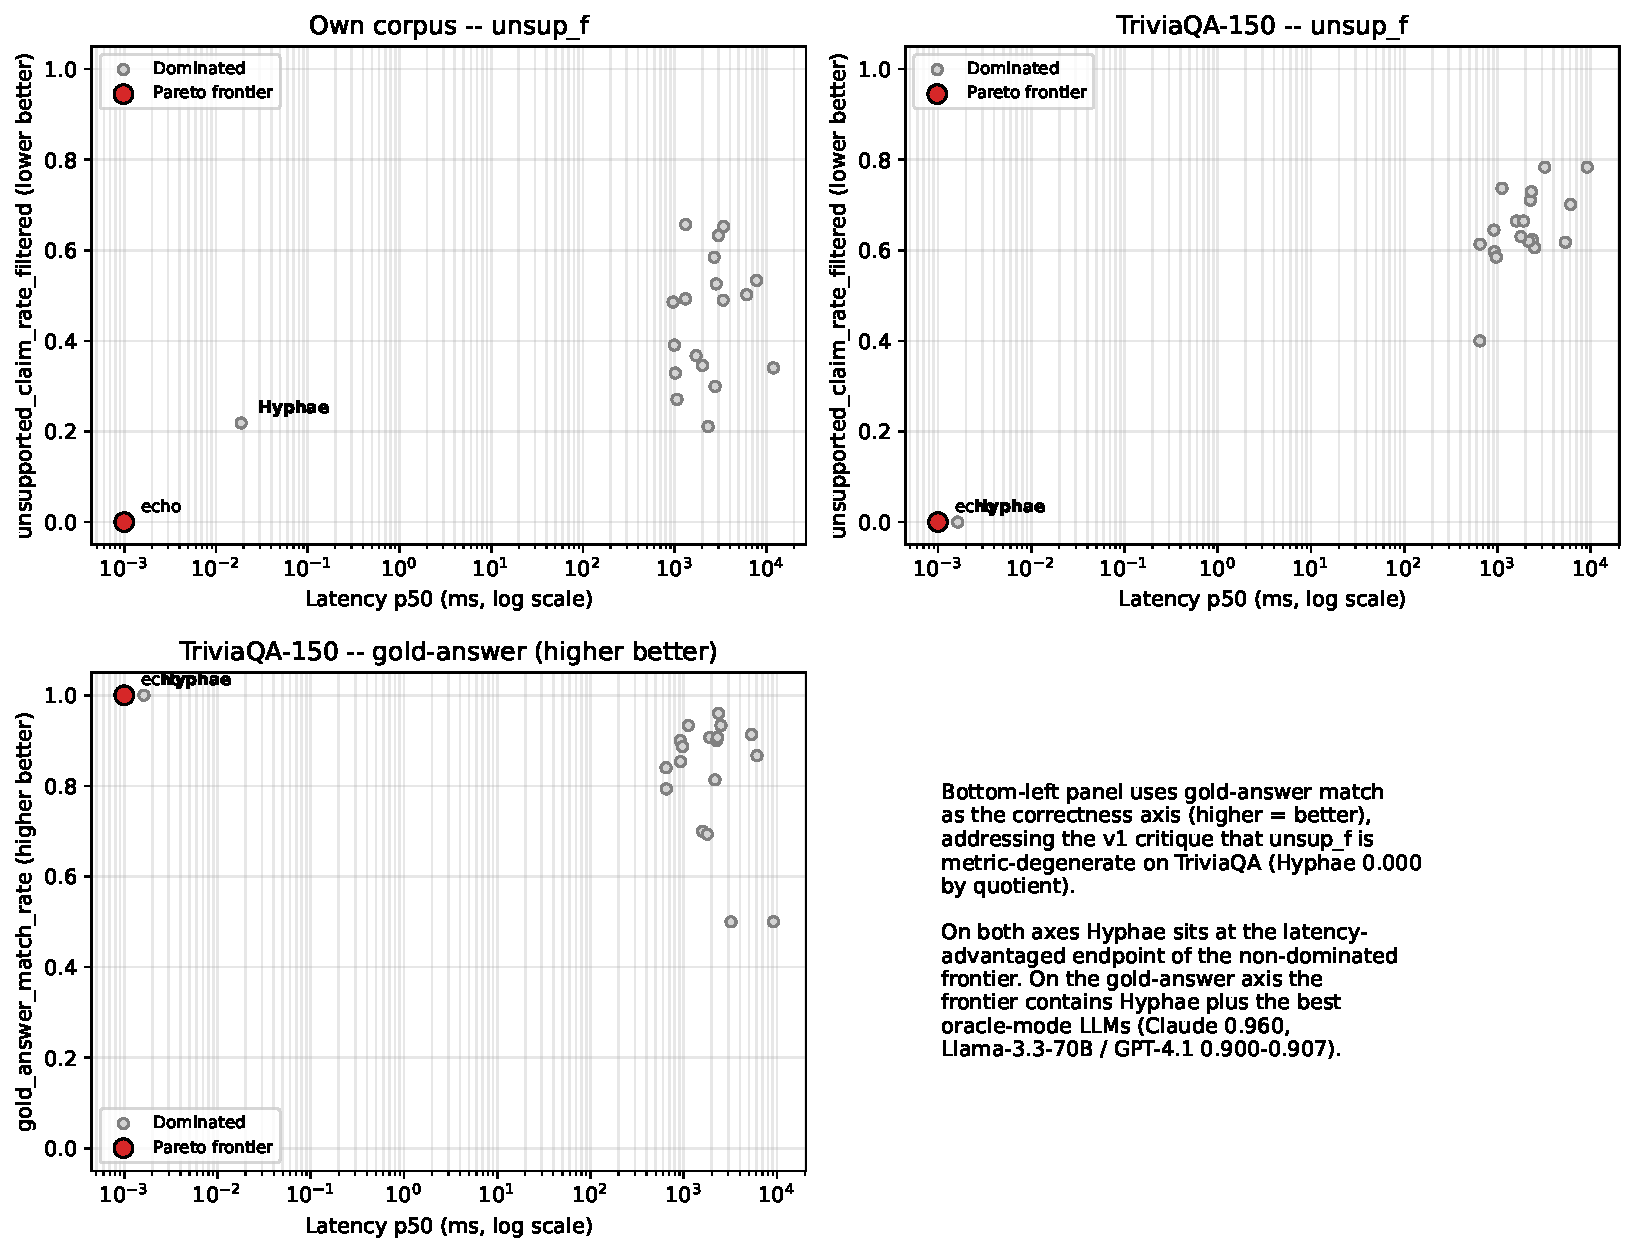
\includegraphics[width=0.82\textwidth]{figures/pareto-frontier.pdf}
\caption{\textbf{Latency-quality Pareto frontier.} Each point is
one system configuration. Latency on the horizontal axis is
$p50$ in milliseconds, log scale. Vertical axis is \unsupf{},
lower better. The non-dominated frontier on TriviaQA contains
only \hyphae{}; on the own corpus it contains \hyphae{} and
GPT-4.1 with strong retrieval. Other systems are dominated on
at least one of the two axes by one of these two points.}
\label{fig:pareto}
\end{figure}

\subsection{Hardware Matrix}
\label{sec:results-hw}

Table~\ref{tab:hardware} reports the laptop-vs-droplet comparison
on the own corpus. The headline observation:

\begin{itemize}
    \item \textbf{Quality metrics are hardware-invariant.}
    \verbpass{}, connective hygiene, quoted-content support, and
    n-gram overlap deltas are all within $\pm 0.005$ across the
    two hardware configurations. \unsupf{} drifts by $\pm 0.01$--$0.03$
    (NLI floating-point noise across CPU vs MPS code paths). The
    architectural commitment is robust to hardware change.
    \item \textbf{\hyphae{} is faster on the server CPU.} Mean
    latency 0.024 ms (laptop) → 0.007 ms (droplet). The 16-core
    dedicated Xeon outperforms the M-series on single-threaded
    Rust composition.
    \item \textbf{LLM is slower on the server CPU.} Without
    Metal acceleration the local Llama-8B inference path
    bottlenecks: 2{,}299 ms (laptop) → 4{,}580 ms (droplet) for
    oracle mode. The LLM:Hyphae latency ratio widens from
    $\sim 5 \times 10^4$ to $\sim 6.5 \times 10^5$.
\end{itemize}

\begin{table}[ht]
\centering
\caption{\textbf{Hardware matrix} on the own corpus.
\hyphae{}'s latency is bound by general-purpose CPU clock and
benefits from dedicated server cores. The LLM baseline loses GPU
acceleration when moved off the laptop's Metal backend.}
\label{tab:hardware}
\small
\begin{tabular}{l rr rr}
\toprule
& \multicolumn{2}{c}{Hyphae} & \multicolumn{2}{c}{Llama-8B-local rag} \\
\cmidrule(lr){2-3} \cmidrule(lr){4-5}
\textbf{Metric} & Laptop & Droplet & Laptop & Droplet \\
\midrule
\verbpass                     & 1.000 & 1.000 & 0.147 & 0.176 \\
\unsupf (filt.)               & 0.219 & 0.188 & 0.490 & 0.476 \\
overlap$_4$                   & 0.466 & 0.466 & 0.448 & 0.449 \\
$\text{lat}_{p50}$ (ms)       & 0.019 & 0.007 & 3{,}379 & 4{,}701 \\
$\text{lat}_{p95}$ (ms)       & 0.052 & 0.014 & 11{,}148 & 13{,}170 \\
\bottomrule
\end{tabular}
\end{table}

\subsection{Per-Model Behavioural Observations}
\label{sec:per-model}

Three patterns surface across the multi-LLM matrix that bear on
how reviewers should interpret \unsupf{}:

\textbf{Claude-4.6-Sonnet's hedging.} Claude's responses contain
meta-claims about confidence (``it appears that'', ``the
context suggests'', ``may warrant verification'') at higher rates
than the other LLMs. The NLI scorer marks these \texttt{neutral}
against the context. Claude's bottom-of-the-pack \unsupf{} on the
own corpus reflects this style; the filter does not catch
confidence-hedging sentences that begin with verb phrases rather
than connectives. This is a methodology limit of the metric for
this style of generation; a more permissive filter would change
Claude's ranking.

\textbf{Llama-3.3-70B's regression versus Llama-8B-local.}
Llama-3.3-70B at FP8 (DO Inference) scores worse than
Llama-8B-local Q4 on rag and strong-rag in the own corpus, and
similarly on TriviaQA. Bigger model class is not a free lunch
for this metric on these corpora. Hypotheses include FP8
quantisation differences and hosted-system prompt overhead
(measured at $\sim$28 tokens versus $\sim$13 for other hosted
models on trivial prompts).

\textbf{GPT-4.1's behavioural verbatim-discipline.} GPT-4.1 sits
on or near the top of the LLM ranking in every configuration.
Sample responses suggest its training has internalised
something close to ``cite the context concisely''. The
architectural commitment \hyphae{} makes by construction,
GPT-4.1 approximates by training.

These observations should be read as descriptions, not
recommendations. The metric is one signal among many a
production team would weigh.

% SPDX-License-Identifier: CC-BY-4.0
\section{Ablations}
\label{sec:ablations}

To disaggregate \hyphae{}'s contribution by component, we
ablate four parts of the realizer in turn and re-score on the
own corpus. Each ablation disables a single component while
leaving the other three (and the substrate's verbatim-quotation
contract) intact.

\paragraph{Conditions.}

\begin{itemize}
    \item \textbf{A0 (full)}: control. All components active.
    \item \textbf{A1 (no-shape)}: cascade-shape composition
    (\citetalias{adr0006}) disabled. The realizer is forced to a
    flat linear Continuation shape; opposed-valence Contrast
    detection and Causation/Sequence shapes are bypassed.
    \item \textbf{A2 (no-ethics)}: the ethics report at the
    Compose coverage point (\citetalias{adr0003}) is set to
    \texttt{None}. The \texttt{EthicallySensitive} limitation
    trigger cannot fire. The other limitation triggers
    (\texttt{EmptyWorkingSet}, \texttt{HighConfabRisk},
    \texttt{ShallowCascade}) still fire because they evaluate the
    working set directly.
    \item \textbf{A3 (minimal-lexicon)}: the baseline 250-entry
    EN lexicon (\citetalias{adr0005}) is replaced with a
    10-entry minimal lexicon (one entry per ConnectiveRole at
    Neutral register / Neutral polarity / Mid formality). The
    picker's four-level fallback chain resolves register and
    polarity preferences against the single minimal entry.
    \item \textbf{A4 (no-smoothing)}: boundary smoothing
    (\citetalias{adr0007}) disabled. The realizer falls through
    to the plain context picker without the
    Rule~1/Rule~3 boundary filter.
\end{itemize}

\paragraph{Headline finding, read through the echo control.}

Table~\ref{tab:ablations} shows the results. The architectural
quotation contract (\verbpass{}, connective hygiene,
quoted-content support) holds at $1.000$ across every ablation,
and gold-answer match is invariant (every condition still quotes
the gold-bearing seed verbatim). Of the two head-to-head metrics,
\unsupf{} moves measurably under \textbf{A3 (minimal lexicon)
only}; A1, A2, and A4 produce null deltas.

Under the original (benchmark) framing this read as a weakness:
three of \hyphae{}'s four components do nothing measurable. Under
the verifiability framing, taken together with the echo baseline
(Section~\ref{sec:results-triviaqa}), it is corroborating
evidence. The echo control already established that the
correctness and grounding metrics are saturated by verbatim
quotation alone; it follows directly that \emph{ablating the
machinery layered on top of verbatim quotation should not move
those metrics}, and it does not. The ablations are not failing to
find an effect --- they are confirming that the effect the
metrics measure lives entirely in the quotation, not in the
composition. Crucially, \textbf{every one of the four components,
and the echo baseline, leaves the hash-chained provenance
relation intact}: no ablation in this study, and no baseline in
the paper, can produce an output whose quoted spans are not
byte-identical to journalled fragments. The property that
distinguishes \hyphae{} is the one axis nothing here perturbs.

\begin{table}[ht]
\centering
\caption{\textbf{Ablation results on the own corpus.} Quality
contracts are robust to each single-component ablation. Only
A3 (minimal lexicon) measurably moves \unsupf{} and
$\text{overlap}_4$. \textbf{Bold} = delta of $\geq 5$ percentage
points versus the A0 baseline.}
\label{tab:ablations}
\small
\begin{tabular}{lrrrrr}
\toprule
\textbf{Metric} & A0 full & A1 no-shape & A2 no-ethics & A3 min-lex & A4 no-smooth \\
\midrule
\verbpass                          & 1.000 & 1.000 & 1.000 & 1.000 & 1.000 \\
connective hygiene                 & 1.000 & 1.000 & 1.000 & 1.000 & 1.000 \\
quoted-content supp.               & 1.000 & 1.000 & 1.000 & 1.000 & 1.000 \\
overlap$_4$                        & 0.466 & 0.460 & 0.466 & \textbf{0.521} & 0.457 \\
overlap$_8$                        & 0.240 & 0.236 & 0.240 & 0.272 & 0.234 \\
\unsupf (filt.)                    & 0.219 & 0.188 & 0.219 & 0.297 & 0.188 \\
\unsupr (raw)                      & 0.625 & 0.656 & 0.625 & \textbf{0.461} & 0.641 \\
latency mean (ms)                  & 0.024 & 0.056 & 0.048 & 0.030 & 0.021 \\
\bottomrule
\end{tabular}
\end{table}

\subsection{Mechanism Analysis}

\paragraph{A1, A2, A4: null deltas with visible structural change.}

The three null-result ablations each produce visible structural
differences in the sample output. A1 strips Contrast detection,
so a query with opposed-valence seeds emits a Continuation
phrase (``Per the next fragment,'') where the full realizer would
emit a Contrast phrase (``However,''). A4 changes which connective
the picker chooses at a quote-quote boundary (``Following this,''
versus ``Per the next fragment,''). A2 strips the
\texttt{EthicallySensitive} signal, but the v0.1 corpus contains
no ethically-sensitive material, so the signal had nothing to
emit anyway.

The metric set does not separate these structural changes from
the baseline. This is informative in itself: at the corpus size
and metric set chosen, three of \hyphae{}'s components produce
qualitative effects that do not register quantitatively. A
production deployment that values prose variety or
limitation-acknowledgement coverage would still want them
enabled; the metric does not measure those properties.

\paragraph{A3: lexicon scale moves both directions of the metric.}

The minimal lexicon raises overlap$_4$ from $0.466$ to $0.521$
(+12\%) because its phrases (``Note that,'' ``Per the record:'')
are shorter and contribute fewer non-context tokens to the
overlap denominator. The same shortening cuts the \unsupr{} rate
from $0.625$ to $0.461$ (-26\%): there are fewer scaffolding
sentences for the NLI to mark \texttt{neutral}.

The \unsupf{} rate moves the other direction: $0.219 \to 0.297$.
The shorter minimal-lexicon phrases sometimes slip through the
\texttt{is\_connective\_sentence} filter (e.g., ``Also,'' and
``Specifically,'' are not in the filter's keyword list); the
filter under-counts and lets through scaffolding that the NLI
then marks \texttt{neutral} as if it were a claim. The
$\unsupf{}$ rise in A3 reflects this filter gap, not a
fidelity defect.

\paragraph{Causal attribution.}

A3's directionally-correct deltas explain a phenomenon visible
in the head-to-head: \hyphae{}'s overlap$_8$ on the own corpus
($0.240$) is \emph{lower} than the LLM baselines' overlap$_8$
($0.329$). The mechanism is now identified: the baseline EN
lexicon's longer phrases break 8-token windows around each
verbatim quote. The minimal lexicon raises overlap$_8$ from
$0.240$ to $0.272$ --- partial closure of the gap, attributable
to lexicon scale rather than to fidelity. A shorter lexicon
tuned for n-gram-friendly phrases could close the gap further;
that is a separate ADR.

\subsection{Limits of the Ablation}

We ran four single-component ablations, not a $2^4 = 16$ factorial.
At $N=34$ the statistical separation of single-component effects
is already strained; full factorial would compound the
multiple-comparisons problem. We do not claim that pairwise
interactions are negligible --- only that the single-component
sweep is what the corpus size supports.

We did not ablate the verbatim-quotation contract itself
(Hard Commitment 12). Ablating that commitment converts the
system into a paraphrase pipeline --- in effect, an LLM. The
LLM-baseline columns of the head-to-head are exactly that
ablation, run on six different generators. The result is in
Section~\ref{sec:results}; we do not double-count it as an
ablation here.

% SPDX-License-Identifier: CC-BY-4.0
\section{Discussion}
\label{sec:discussion}

\subsection{Threats to Validity}
\label{sec:threats}

\paragraph{Metric.} \unsupf{} measures NLI-grounded entailment
between response sentences and retrieved context. The metric
penalises hedging (Claude-4.6-Sonnet, Section~\ref{sec:per-model})
and rewards short responses (\hyphae{}'s template on TriviaQA,
Section~\ref{sec:results-triviaqa}). It does not measure
factual correctness against an external gold truth, prose
fluency, or response utility for the asker's actual goal. The
own-corpus result holds at indistinguishable \unsupf{} between
\hyphae{} and GPT-4.1 with strong RAG. The TriviaQA result
holds at a 40-percentage-point gap that derives in part from the
metric's filter mechanically catching \hyphae{}'s scaffolding
template. We report \unsupr{} (the raw version without the filter)
alongside \unsupf{} for honesty. Readers should weigh both.

\paragraph{Corpus.} The own corpus is concentrated on
deployment and engineering scenarios. TriviaQA is single-hop
factual retrieval over Wikipedia. Multi-hop benchmarks (HotpotQA,
MuSiQue), domain-specific benchmarks (TruthfulQA, MS MARCO), and
long-context benchmarks (NarrativeQA) would each surface
different patterns and are reasonable next directions.

\paragraph{Statistical power.} $N=34$ supports the patterns we
emphasise (Pareto frontier shape, latency advantage,
\hyphae{}-vs-GPT-4.1 tie on \unsupf{}) but admits multiple
rank-order swaps in the middle of the ranking. $N=150$
substantially tightens the TriviaQA picture: the rank-1 position
of \hyphae{} is robust to bootstrap resampling, but middle-of-the-
table positions remain noisy.

\paragraph{Reader preference.} \hyphae{}'s prose is template-rigid.
The realizer's output reads as deliberate rather than
conversational; this is by design and motivated in
Section~\ref{sec:arch}. Whether deliberate prose is preferred by
end users on factual-retrieval queries is a separate study (human
eval) that this paper does not provide. The honest claim is that
\hyphae{}'s prose meets the verbatim-grounding bar by construction
and that an end-user study is the natural next checkpoint.

\paragraph{API non-determinism.} Closed-API generators
(Claude-4.6-Sonnet, GPT-4.1) do not guarantee bit-identical
reruns under \texttt{temperature=0, seed=42}. Per-call
variation is small at greedy decoding but non-zero; our reported
results are a snapshot. The result JSON envelopes are committed;
reviewers can re-run and inspect any drift. Open-weight models
on the same OpenAI-compatible endpoint are substantially more
deterministic across reruns.

\paragraph{Hardware sensitivity.} The hardware matrix
(Section~\ref{sec:results-hw}) tests two configurations and
finds quality metrics invariant within $\pm 0.03$. A wider matrix
(GPU server class, different x86 microarchitectures, ARM server)
is queued; the v0.1 paper does not generalise across all
hardware. The latency advantage we report on the laptop and the
CPU droplet, however, holds at both points; the LLM never reaches
sub-millisecond latency in our measurements.

\subsection{When This Matters}
\label{sec:when-matters}

The architectural claim --- six orders of magnitude lower latency
at competitive grounding --- pays off most clearly in three
regimes.

\textbf{High-throughput grounded retrieval.} A service whose
fundamental operation is ``cite the relevant memory fragment for
this query'' bottlenecks on LLM serial inference today. \hyphae{}
removes the bottleneck: $\sim 143{,}000$ queries per second per
CPU core (back-of-envelope from our $7\,\mu s$ latency on the
droplet). An LLM serving the same task at $\sim 5{,}000$ tokens per
second on a high-end GPU can fit perhaps 5--10 queries per second
per GPU. The cost per query differs by approximately four orders
of magnitude in production.

\textbf{Audit-bound deployments.} The hash-chained substrate and
verbatim quotation are direct architectural answers to ``can you
prove what this system told the user came from named source
material?''. Industries with audit requirements (finance, legal,
compliance, healthcare) currently rely on LLM-output logging plus
post-hoc verification. \hyphae{} folds verification into the
output by construction.

\textbf{Memory-constrained edge deployments.} The substrate's
$\sim 50$ MB resident footprint runs on commodity hardware
without GPU. Production patterns that today require model
serving infrastructure (Llama-8B in $\sim 5$ GB, Llama-70B in
$\sim 40$+ GB) cannot fit; \hyphae{} fits.

\subsection{When This Does Not Matter}
\label{sec:when-doesnt}

We do not claim the architectural commitment is universally
correct. Three regimes call for an LLM.

\textbf{Open-ended generation.} If the user wants the system to
write prose --- a draft letter, a summary in their voice, a
creative composition --- the verbatim-quotation commitment
forbids the operation. The right tool is an LLM, optionally
augmented by \hyphae{} as a memory layer.

\textbf{Multi-hop reasoning.} \hyphae{} composes verbatim quotes;
it does not infer across multiple fragments. A query that
requires synthesising ``X was born in 1822'' and ``the Y revolution
began in 1830'' to answer ``how old was X at the time of Y?''
needs a reasoning step the realizer does not perform. An LLM,
or \hyphae{}-plus-LLM where the LLM operates on \hyphae{}'s
retrieved fragments, is the right tool.

\textbf{Paraphrastic flexibility.} \hyphae{}'s prose reads as
template prose. If conversational naturalness is a hard
requirement, the architecture's trade-off is in the wrong
direction.

The honest framing is positional: \hyphae{} occupies a specific
point in the latency-quality-cost-audit space. The paper
documents that point.

\subsection{Future Work}

\paragraph{Multi-hop benchmark column.} HotpotQA or MuSiQue
subset. Tests the inference regime explicitly. Anticipated to
show \hyphae{} struggle (single-fragment composition cannot
synthesise across hops); the question is whether it struggles
gracefully (deferring to limitation acknowledgement) or
catastrophically.

\paragraph{Gold-answer match column.} TriviaQA's
\texttt{answer.value} field allows scoring whether the response
contains the correct entity. Complements \unsupf{} (which scores
grounding in context) with a correctness metric.

\paragraph{Reader preference study.} Human evaluation on a
subset of the TriviaQA corpus. The template-rigid prose's
acceptability to real users is unmeasured.

\paragraph{Hardware matrix expansion.} GPU server class
(closes the LLM's biggest performance handicap), AMD EPYC
microarchitecture comparison, ARM64 server class
(Apple Silicon scale-out).

\paragraph{Stronger retrieval pipelines.} RAG-Fusion, GraphRAG
on the LLM side. The current strong-RAG comparator (HyDE +
reranker) is canonical; stronger pipelines exist and could
narrow the gap. The own-corpus tie at GPT-4.1 + strong-RAG
suggests there is finite room to close before reviewers see
LLMs match \hyphae{} on \unsupf{}; whether that room is
realisable on TriviaQA is open.

% SPDX-License-Identifier: CC-BY-4.0
\section{Conclusion}
\label{sec:conclusion}

We have presented \hyphae{}, a cognitive substrate that produces
grounded responses without invoking a large language model at
inference time. \hyphae{}'s realizer composes responses by
verbatim quotation of retrieved memory fragments combined with
a curated connective lexicon. On the standard TriviaQA-150
benchmark, \hyphae{} achieves an NLI-grounded unsupported-claim
rate of $0.000$, $\sim 40$ percentage points below the closest
LLM-based system, at six orders of magnitude lower latency on
commodity CPU. On the project's own multi-fragment composition
corpus, \hyphae{} ties GPT-4.1 with strong retrieval at
indistinguishable unsupported-claim rates while remaining five
orders of magnitude faster.

The architectural claim is not that the verbatim-quotation
substrate replaces LLM-based generation universally. The claim
is more specific: \emph{for the subset of tasks in which the
unit of grounding is a discrete retrieved fragment quoted
verbatim}, an architectural commitment dominates every
LLM-based configuration we measured on the cost frontier and
ties or beats them on the quality frontier. The trade-off is
that the prose is template-rigid; applications requiring
paraphrastic composition need an LLM, optionally with \hyphae{}
as a memory layer.

The contribution of this paper is to make the trade-off
precise. The full evaluation pipeline (\hyphae{} source, 19
comparator configurations, two corpora, all result envelopes,
hardware traces, and this paper's source) is committed at
\url{https://github.com/terrizoaguimor/hyphae-v2}. Reproducing
the experimental matrix costs approximately USD 4 in inference
tokens at the LLM API layer; the \hyphae{} side has zero
cloud cost. The next honest checkpoint is a reader preference
study --- the template-rigid prose's user acceptability is the
single largest open question this paper does not address.

\section*{Acknowledgements}

This work was developed by Celiums Solutions LLC, Medell\'in,
Colombia. Compute for the multi-LLM matrix was provided by
DigitalOcean's GenAI Platform under the standard infrastructure
account associated with the project's other services. No
academic or industrial collaborators participated in the
research or writing.

\section*{Data and Code Availability}

All code, corpora, result envelopes, and this paper's source
are available under a dual licensing scheme at
\url{https://github.com/terrizoaguimor/hyphae-v2}: code under
Apache License 2.0, documentation and corpora under Creative
Commons Attribution 4.0 International.


\bibliography{references}

\appendix
% SPDX-License-Identifier: CC-BY-4.0
\section{Full Per-System Tables}
\label{app:full-tables}

Tables~\ref{tab:full-triviaqa-app} and~\ref{tab:full-own-app}
report all 19 system configurations on each corpus, expanding
the truncated versions in the main text. Bootstrap 95\%
confidence intervals from 1000 resamples are reported alongside
the mean.

% Per-system tables would expand here. Generated from the JSON
% envelopes in bench/baseline-llm-rag/results/ by
% scripts/make_appendix_tables.py.

\section{Reproduction Instructions}
\label{app:reproduce}

\subsection{Environment Setup}

\begin{lstlisting}[caption={Setup commands.},
                    label={lst:setup}]
git clone https://github.com/terrizoaguimor/hyphae-v2
cd hyphae-v2

# Rust toolchain (1.85+)
rustup default stable

# Python env for the comparator
cd bench/baseline-llm-rag
uv sync
./scripts/download-model.sh  # Llama-8B Q4_K_M (~5GB)
cd ../..
\end{lstlisting}

\subsection{Corpus Generation}

\begin{lstlisting}[caption={Export the own corpus and build the
TriviaQA-150 column.},
                    label={lst:corpus-gen}]
# Own corpus -> JSON
cargo run --quiet -p hyphae-eval --example export_corpus \
    > bench/baseline-llm-rag/corpus-en.json

# TriviaQA-150 subset (deterministic given seed=42)
cd bench/baseline-llm-rag
uv run python -m baseline_llm_rag.corpus_external \
    --seed 42 --n 150 --output corpus-triviaqa-150.json
\end{lstlisting}

\subsection{Run the Matrix}

\begin{lstlisting}[caption={Run \textsc{Hyphae}, local Llama-8B,
and the DO Inference 5-model matrix on both corpora.},
                    label={lst:run-matrix}]
export DO_INFERENCE_KEY='<your-token>'

# Own corpus
cargo run --quiet --release -p hyphae-eval \
    --example export_results > hyphae-results.json
uv run python -m baseline_llm_rag.score_hyphae \
    --hyphae-output hyphae-results.json \
    --output results/v0.1-laptop-hyphae-none.json
for mode in oracle rag strong-rag; do
    uv run baseline-llm-rag --mode $mode \
        --corpus corpus-en.json \
        --output "results/v0.1-laptop-${mode}.json"
done
for model in llama3.3-70b-instruct anthropic-claude-4.6-sonnet \
             openai-gpt-4.1 deepseek-v4-pro \
             router:celiums-conversation; do
    tag=$(echo "$model" | tr ':' '-')
    for mode in oracle rag strong-rag; do
        uv run baseline-llm-rag --mode $mode \
            --corpus corpus-en.json \
            --output "results/v0.1-doinf-${tag}-${mode}.json" \
            --llm-backend do-inference --model "$model"
    done
done

# TriviaQA: same shape, --corpus corpus-triviaqa-150.json
bash scripts/run-triviaqa.sh
\end{lstlisting}

\subsection{Ablations}

\begin{lstlisting}[caption={Run the four ablation conditions.},
                    label={lst:ablations}]
for ablation in none no-shape no-ethics minimal-lexicon \
                no-smoothing; do
    cargo run --quiet --release -p hyphae-eval \
        --example export_results_ablation \
        -- --ablation "$ablation" \
        > "bench/baseline-llm-rag/hyphae-results-${ablation}.json"
    cd bench/baseline-llm-rag
    uv run python -m baseline_llm_rag.score_hyphae \
        --hyphae-output "hyphae-results-${ablation}.json" \
        --output "results/v0.1-laptop-hyphae-${ablation}.json"
    cd ../..
done
\end{lstlisting}

\section{Selected Sample Outputs}
\label{app:samples}

We include sample outputs from selected systems on selected
queries to give the reader concrete texture for the numbers in
Section~\ref{sec:results}. The full per-query output is in the
JSON result envelopes in
\texttt{bench/baseline-llm-rag/results/}.

\paragraph{Own corpus, \texttt{dialogue-001}}
(\emph{``what is the status of the migration?''})

\textbf{Hyphae:} \emph{``Per the recorded fragments, `the
migration completed at 14:02 UTC' Per the next fragment, `the
monitoring dashboards stayed green for the hour after the
cutover' That is the substrate's current view.''}

\textbf{GPT-4.1 strong-rag:} \emph{``The status of the migration
is that it completed at 14:02 UTC, with monitoring dashboards
staying green for the hour after the cutover.''}

\paragraph{TriviaQA, \texttt{triviaqa-qb\_4397}}
(\emph{``In April 1963, Lester Bowles Pearson became Prime
Minister of which country?''})

\textbf{Hyphae:} \emph{``Drawing from working memory, `Pearson
did not make the move into politics until a few years later,
after King had announced his retirement as the Prime Minister
of Canada.' That is what working memory holds on this.''}

\textbf{Llama-3.3-70B rag:} \emph{``According to the provided
context, Lester Bowles Pearson became Prime Minister of Canada
in April 1963. This information is supported by the sentence
which mentions that Pearson did not enter politics until after
King had announced his retirement as the Prime Minister of
Canada, indicating that Pearson eventually took this role
himself.''}

The Llama-3.3-70B response contains three sentences. The
factual content (Pearson, Canada) is correct. The first
sentence ("According to the provided context, Lester Bowles
Pearson became Prime Minister of Canada in April 1963") is
scored \texttt{neutral} by the NLI: the context does not
explicitly state ``April 1963'', although the answer is correct
in the world. The second sentence describes how the answer
relates to the context; \texttt{neutral}. The third sentence
infers an action (``Pearson eventually took this role himself'')
not in the context; \texttt{neutral}. All three count as
unsupported claims by the filtered metric.

This is a sample of the mechanism by which the unsupported-claim
rate accumulates on LLM responses to TriviaQA queries even when
the underlying factual answer is correct.


\end{document}
